\newcommand\scaleVal{0.45}

\begin{frame}{Database points -- \Romannum{1}}

    \begin{columns}
        \column{0.5\textwidth}
        \begin{figure}
            \centering
            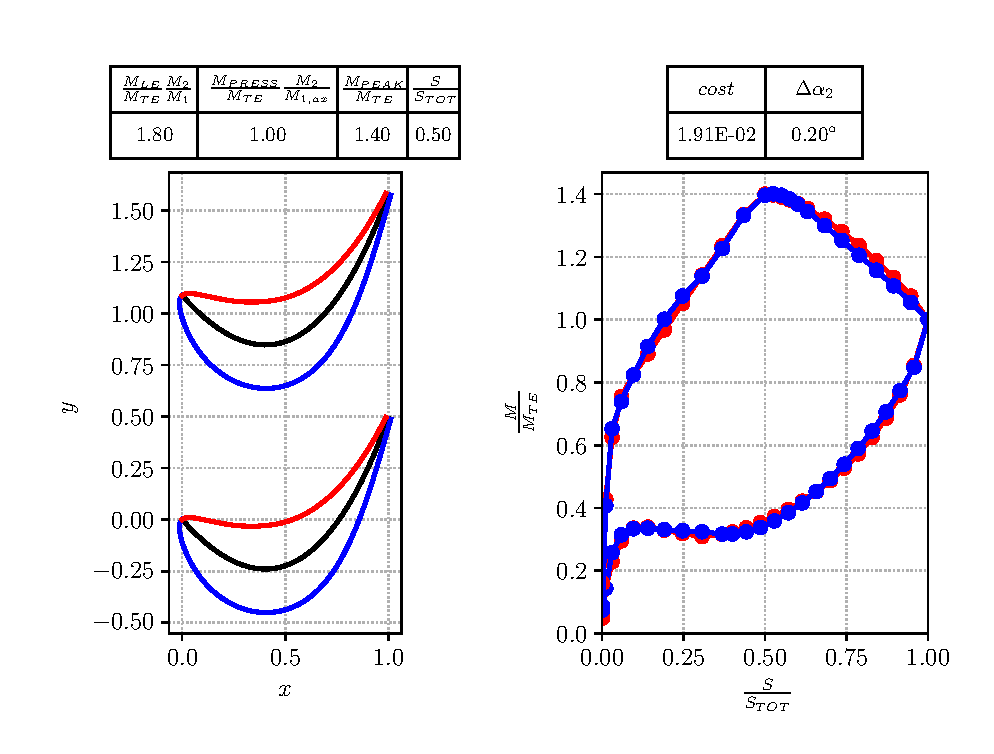
\includegraphics[scale=\scaleVal]{./images/bladeVal0305.eps}
        \end{figure}
        \column{0.5\textwidth}
        \begin{figure}
            \centering
            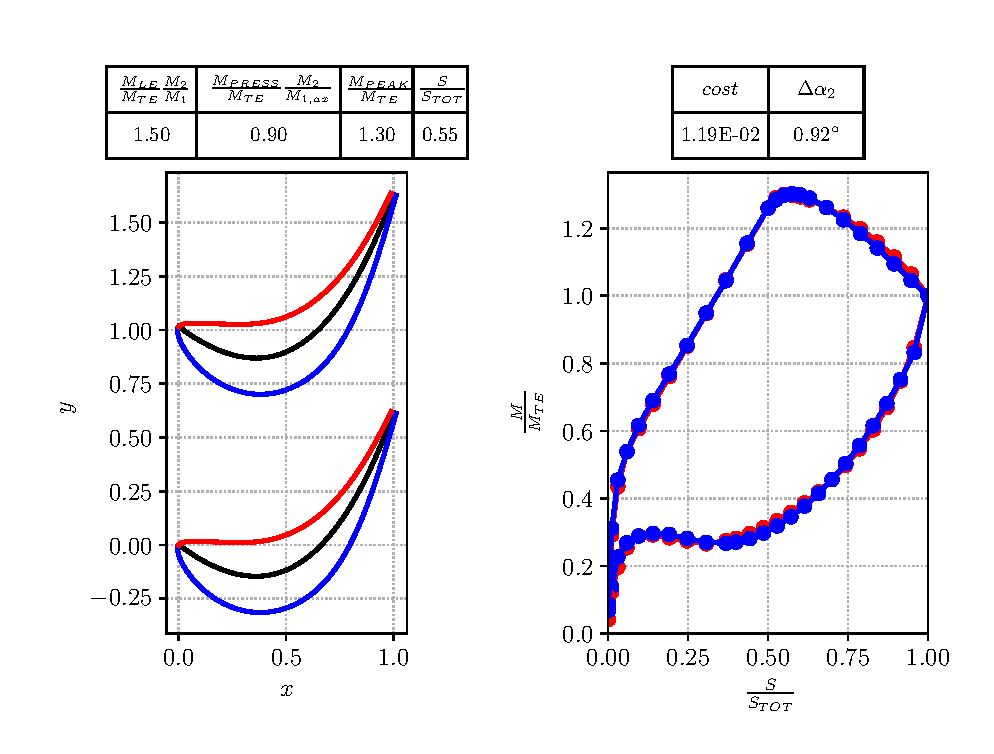
\includegraphics[scale=\scaleVal]{./images/bladeVal1336.eps}
        \end{figure}
    \end{columns}
\end{frame}

\begin{frame}{Database points -- \Romannum{2}}
    \begin{columns}
        \column{0.5\textwidth}
        \begin{figure}
            \centering
            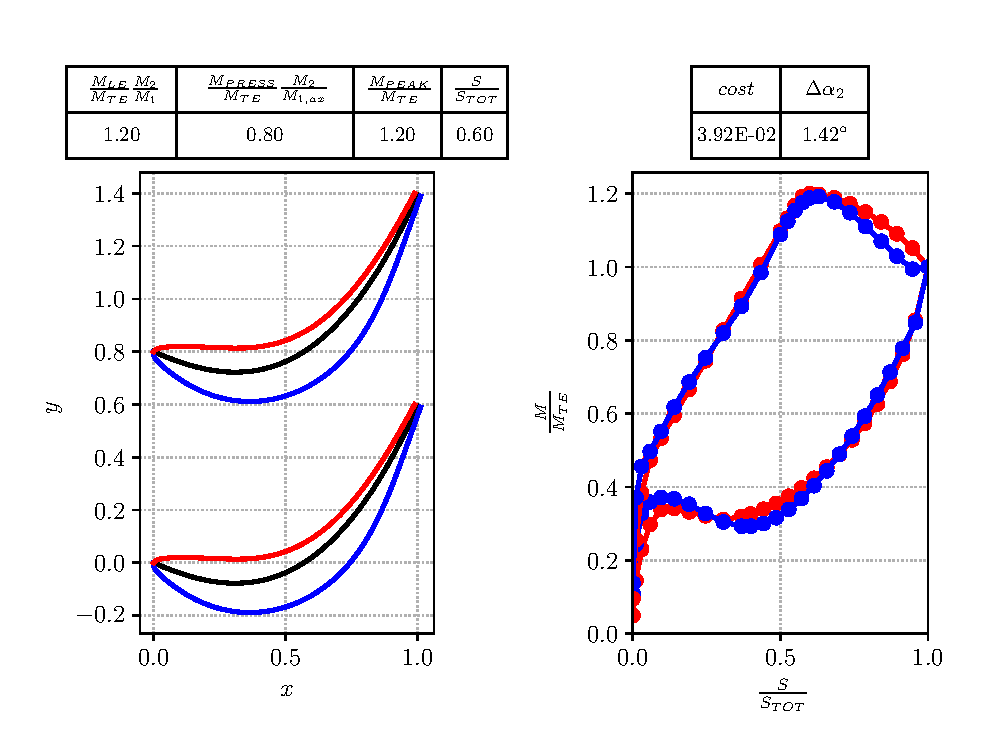
\includegraphics[scale=\scaleVal]{./images/bladeVal1962.eps}
        \end{figure}
        \column{0.5\textwidth}
        \begin{figure}
            \centering
            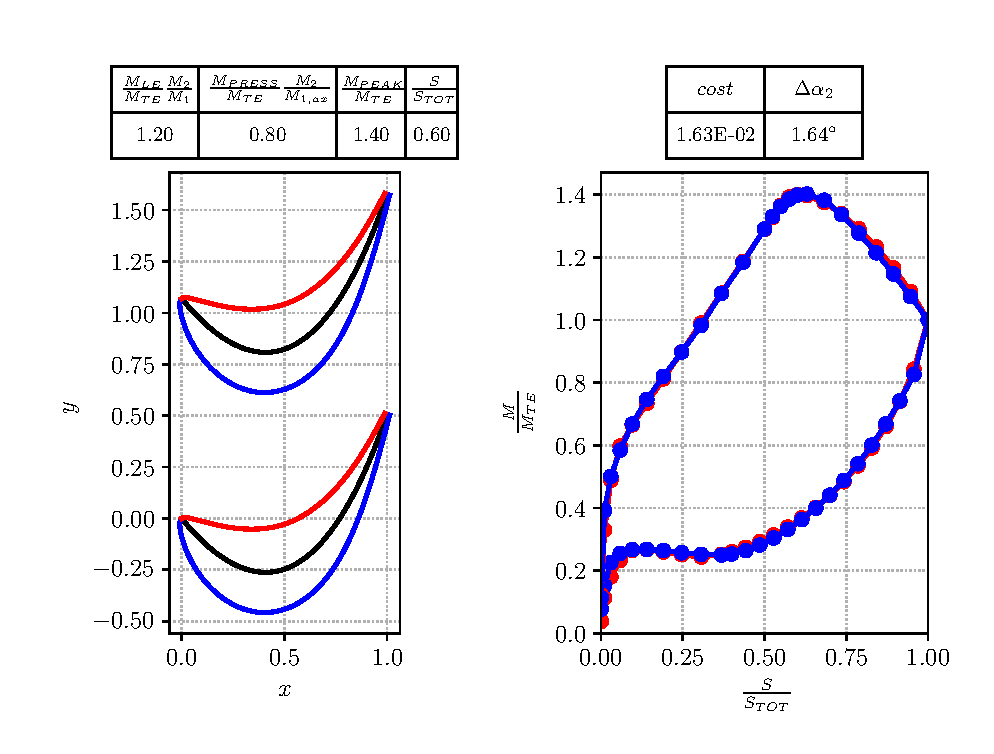
\includegraphics[scale=\scaleVal]{./images/bladeVal0477.eps}
        \end{figure}
    \end{columns}
\end{frame}

% \begin{frame}{Database points -- \Romannum{3}}
%     \begin{columns}
%         \column{0.5\textwidth}
%         \begin{figure}
%             \centering
%             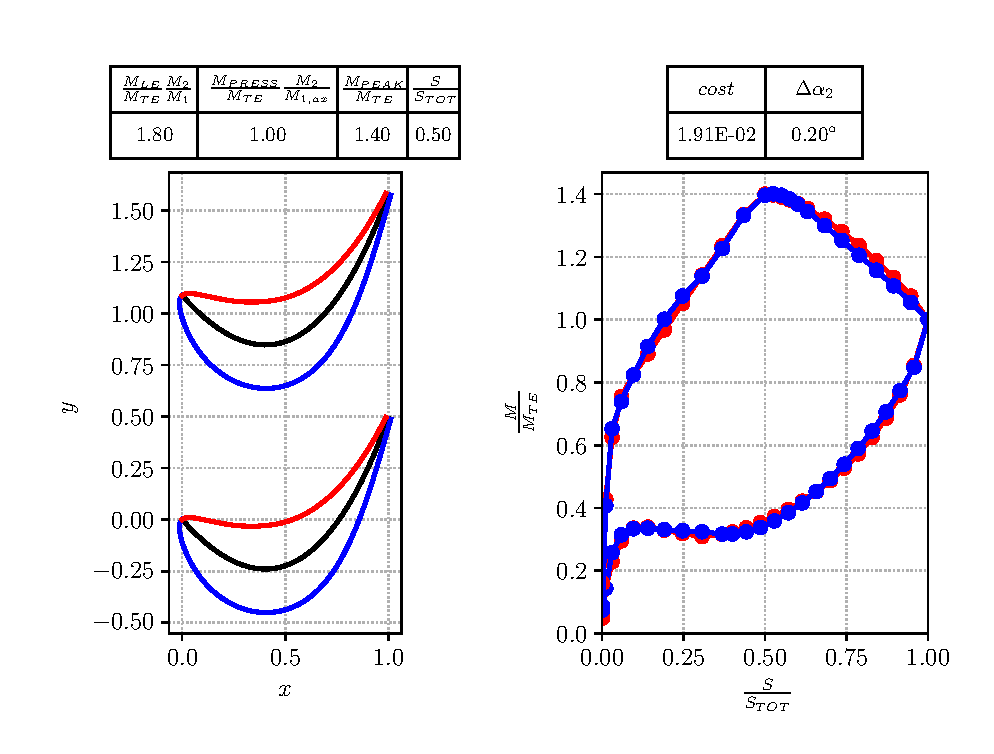
\includegraphics[scale=\scaleVal]{./images/bladeVal0305.eps}
%         \end{figure}
%         \column{0.5\textwidth}
%         \begin{figure}
%             \centering
%             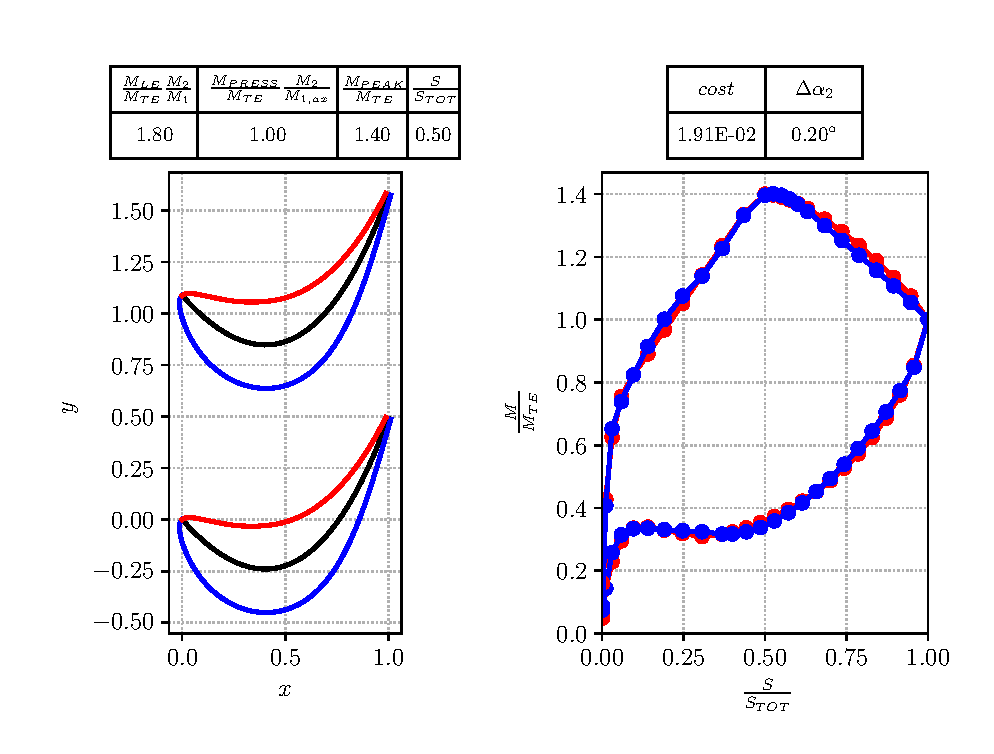
\includegraphics[scale=\scaleVal]{./images/bladeVal0305.eps}
%         \end{figure}
%     \end{columns}
% \end{frame}

\begin{frame}{Errors}
    \begin{columns}
        \column{0.5\textwidth}
        % \vspace{-1.5cm}
        \begin{figure}
            \centering
            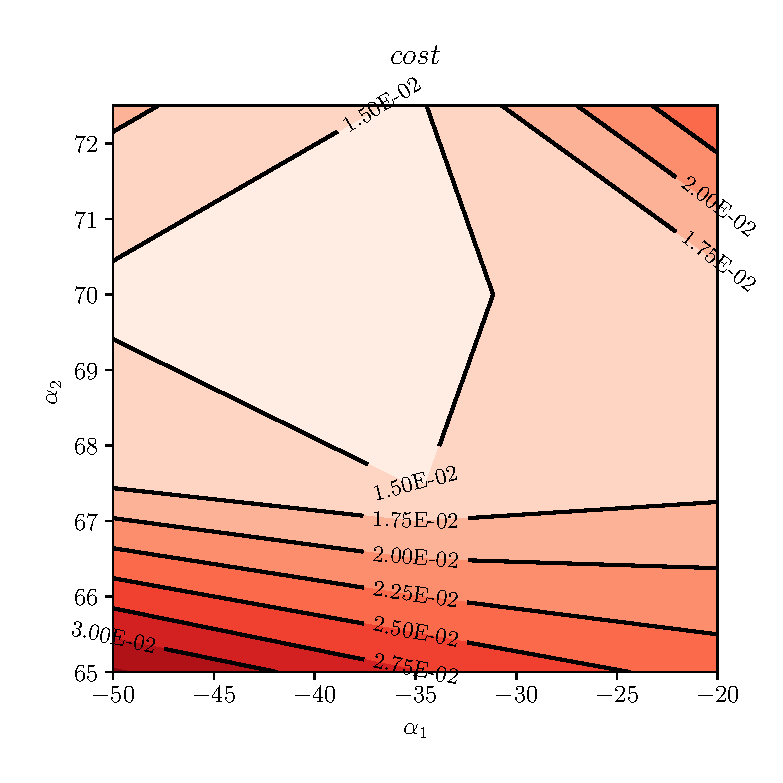
\includegraphics[scale=0.5]{./images/cost.eps}
        \end{figure}
        \column{0.5\textwidth}
        % \vspace{-1.5cm}
        \begin{figure}
            \centering
            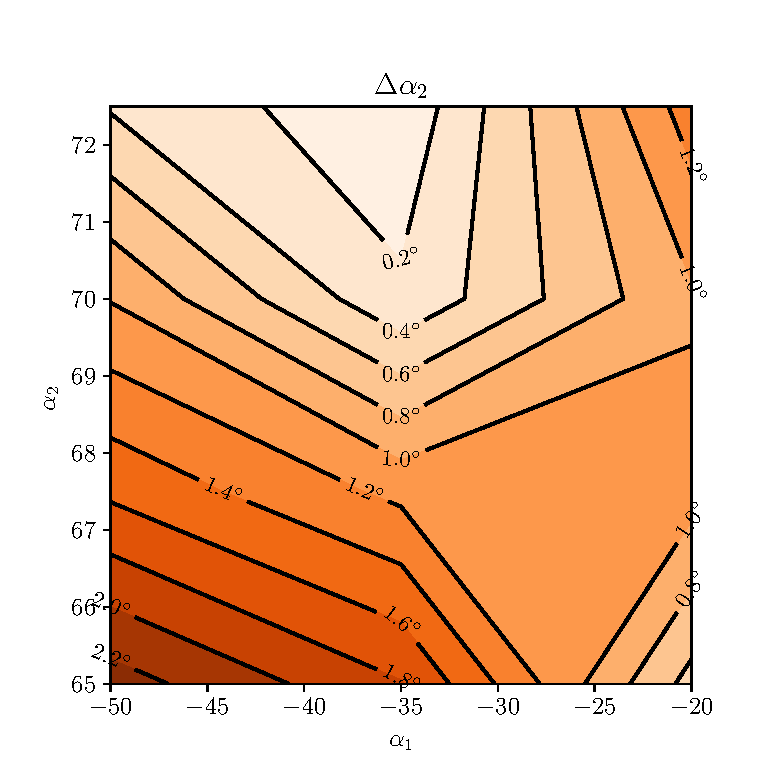
\includegraphics[scale=0.5]{./images/angleError.eps}
        \end{figure}
    \end{columns}
\end{frame}

\begin{frame}{Feasible design}
    \begin{columns}
        \column{0.5\textwidth}
        % \vspace{-1.5cm}
        \begin{figure}
            \centering
            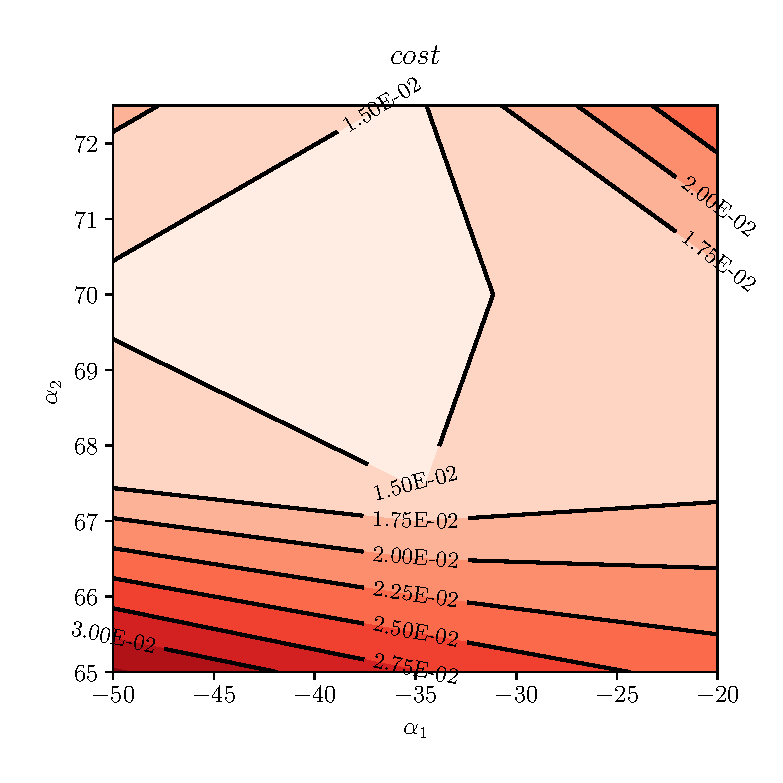
\includegraphics[scale=0.5]{./images/cost.eps}
        \end{figure}
        \column{0.5\textwidth}
        Once the full database has been computed, part of the database is not considered due to the \textbf{poor data quality}. 
        \\[0.5cm]
        Data is considered of poor quality if does \textbf{not satisfy sufficiently well} the \textbf{objectives} and the \textbf{constraints}. 
        \\[0.5cm]
        All these instances will be \textbf{omitted} from the database interpolation using ML. 
        \\[0.5cm]
        This filterning process underlines the \textbf{poor correlation of objectives and constraints} in the domain. 
    \end{columns}
\end{frame}